\documentclass{tmsce}

% ---------------- Packages ----------------
\usepackage{amsmath,amsfonts,amsthm}
\usepackage{array}
\newcolumntype{L}[1]{>{\raggedright\arraybackslash}p{#1}}
\usepackage[caption=false,font=normalsize,labelfont=sf,textfont=sf]{subfig}
\usepackage{textcomp}
\usepackage{stfloats}
\usepackage{url}
\usepackage{graphicx}
\usepackage{longtable}
\usepackage{booktabs}
\usepackage{float}
\usepackage{cite}

\titleformat{\section}
  {\LARGE\bfseries}
  {\thesection}{1em}{}

\titleformat{\subsection}
  {\Large\bfseries}
  {\thesubsection}{1em}{}

\titleformat{\subsubsection}
  {\normalsize\bfseries}
  {\thesubsubsection}{1em}{}

\hyphenation{Poly-market Bin-ance micro-second}

\let\oldsection\section
\renewcommand{\section}{\clearpage\oldsection}

\begin{document}

% ---------------- Title/Author ----------------
\begin{titlepage}
    \vspace*{2.1cm}
    \begin{center}
        {\LARGE\bfseries Low-Latency Cross-Venue Arbitrage:\\[0.4em]
         Binance $\rightarrow$ Polymarket} \\[1.1em]
        {\large Strategy, Infrastructure, Deployment, and a Production Post-Mortem} \\[1.6em]
        {\large Cullen Trace Campana}
    \end{center}
    \vspace{1.9em}
    \begin{center}
    \begin{minipage}{0.86\textwidth}
        \small
        \setlength{\parindent}{0pt}
        \textbf{Abstract.} This report documents the design, deployment, and
        post-mortem of a production, real-money low-latency trading system that
        exploited a repricing lag between Binance spot and Polymarket's short-dated
        crypto prediction markets. The system spans two AWS regions. A Tokyo node
        co-located with Binance detects order-book moves through a three-gate detector
        and transmits a 20-byte, loss-tolerant UDP signal to a Dublin node co-located
        with Polymarket, which validates against the live CLOB and executes
        fill-and-kill orders. Node-internal compute is sub-millisecond (signal-to-wire
        50--200\,\textmu s), and end-to-end latency, dominated by the transatlantic
        hop, was measured at 140--150\,ms, inside the 150--500\,ms window over which
        the target book reprices. Detection is calibrated per asset with Optuna and
        augmented by per-asset LightGBM and random-forest meta-labeling; execution runs
        eight shared-nothing per-asset pipelines behind an explicit per-position state
        machine, a dual-window rate limiter, and a mock-to-live harness with exact API
        parity.
        Across an $8{,}576$-trade replay backtest the strategy won $61.4\%$ with a
        coherent, well-structured microstructure edge (repricing half-life
        ${\approx}\,786$\,ms). Deployed with real capital on ${\sim}\$100$/month of
        infrastructure, it came out effectively flat: the displayed Polymarket depth
        was largely spoofed, so the live fill rate fell to ${\sim}10\%$ against
        ${\sim}100\%$ in paper, and the orders that did fill were close to coin flips.
        The report quantifies and explains this outcome, a market-microstructure limit
        rather than an engineering one, and draws general lessons for latency arbitrage
        against untrusted liquidity.
    \end{minipage}
    \end{center}
    \vfill
\end{titlepage}

\clearpage
\tableofcontents
\clearpage


% =========================================================
\section{Executive Summary}

This report documents a low-latency trading system built to exploit a specific,
well-defined inefficiency: Polymarket's short-dated crypto ``up-or-down''
prediction markets reprice with a measurable lag relative to the underlying spot
price on Binance. The system was engineered to production depth: two co-located
compute nodes in different AWS regions, a hand-rolled 20-byte UDP signalling
protocol, shared-nothing per-asset processing pipelines, a full mock-to-live execution
harness, and per-asset parameter calibration against replayed market data. It was
deployed to AWS and traded with real capital.

\medskip
\noindent In replay, the strategy performed well. Across $8{,}576$ trades drawn from
roughly $52$ hours of recorded order flow, it won $61.4\%$ of the time with a
positively-skewed per-trade P\&L distribution and a stable upward equity curve. The
signal was predictive, the microstructure edge was measurable and decayed as the
thesis predicted, and the performance had sensible internal structure: it was
strongest in quiet books, at prices away from $0.50$, and at short holding periods,
and it weakened in each of the opposite conditions.

\medskip
\noindent It did not survive contact with the live market, and the reason it failed
is the main finding of this report. The latency edge was real and was captured as
designed. What broke the strategy was not speed, model quality, or engineering: it
was that the liquidity it was pricing against did not exist. The displayed depth on
Polymarket's order book was, in large part, spoofed. In paper trading, where fills
were simulated against the \emph{displayed} book, the system filled essentially every
marketable order. In live trading, where fills were matched against \emph{real}
resting size, roughly one order in ten filled, and those fills were close to coin
flips. The edge was priced into a book that disappeared as soon as a real order tried
to cross it. The strategy did not lose money; it simply could not capture the edge it
was built for, and was retired near break-even.

\subsection{The Trade Idea}

Polymarket runs recurring 5-minute and 15-minute markets on whether BTC, ETH, SOL,
or XRP will be higher or lower at the window's close. The fair value of the ``Yes''
(up) token is a monotone function of the current underlying price relative to the
window's reference level and the time remaining. When Binance spot moves, that fair
value changes instantly, but the Polymarket order book does not: quotes are updated
by market makers and arbitrageurs reacting to the same Binance feed, and that
reaction takes an observed 150--500\,ms. The trade is to detect a Binance move,
decide which outcome token it favours, and lift the correct side before the book
reprices.

\subsection{The System}

Detection and execution are geographically separated because the two venues are.
Binance's matching engine is best reached from AWS \texttt{ap-northeast-1} (Tokyo);
Polymarket's CLOB is best reached from AWS \texttt{eu-west-1} (Dublin). A
\textbf{Tokyo} node watches the Binance book and trade streams, runs a three-gate
move detector, and fires a compact UDP signal to Dublin. A \textbf{Dublin} node
receives the signal, checks the live Polymarket book through a set of entry gates,
and executes a fill-and-kill order through an ECDSA-signed CLOB client. The path from
a Binance price move to an order arriving at Polymarket was measured at roughly
140--150\,ms, dominated by the $\sim$120\,ms transatlantic hop between the two nodes.

\subsection{What Was Validated and What Was Not}

The \emph{signal} was validated: recorded data shows Polymarket repricing toward the
signal within the first second or two after a Binance move
(Section~\ref{sec:edge-empirical}), and the backtested strategy was profitable with
coherent conditional structure (Section~\ref{sec:backtest}). The \emph{latency
budget} was validated: the system consistently delivered orders inside the repricing
window. The \emph{execution surface} was not, and could not have been, validated in
paper, because the paper harness inherited the same blind spot that the market
exploited: it trusted the displayed book. This is the central lesson
(Section~\ref{sec:postmortem}).

\subsection{Lessons}

Three conclusions carry beyond this specific strategy. First, in a latency
arbitrage the binding constraint is often not your own speed but the
\emph{realisability} of the liquidity you are racing toward; displayed size is not
the same as available size. Second, a paper-trading harness that simulates fills
against the displayed book will systematically overstate the performance of any
strategy that takes liquidity, because it cannot see cancellation-on-arrival. Third,
geography is a hard constraint: when the price source and the execution venue are on
opposite sides of the world, the transit cost dominates every micro-optimisation, and
local engineering cannot recover it.

\medskip
\noindent\textbf{A note on the data in this report.} Much of the quantitative
material here was reconstructed from recorded feed sessions and a replay backtest
(the \texttt{regime\_trade\_log} and \texttt{edge\_signals} datasets, $8{,}576$
trades and $4{,}892$ signals respectively). All backtest results should be read as
\emph{paper} results under a displayed-liquidity fill assumption; the divergence
between them and the live outcome is the subject of Section~\ref{sec:postmortem}.


% =========================================================
\section{The Trade Idea}
\label{sec:trade-idea}

\subsection{Polymarket Short-Dated Crypto Markets}

Polymarket lists a continuous series of short-horizon binary markets on major
cryptocurrencies. For each asset in \{BTC, ETH, SOL, XRP\} and each timeframe in
\{5\,min, 15\,min\}, a market opens asking whether the asset will close the window
above or below its opening reference. Each market resolves to a pair of outcome
tokens (``Yes'' for up, ``No'' for down) that trade on a central limit order book
priced in the interval $(0,1)$ and settle at \$1 for the correct outcome and \$0 for
the incorrect one. A new window rotates in every 5 or 15 minutes; the system
discovers active windows by constructing the exact market slugs
(\texttt{btc-updown-5m-\{ts\}}) and querying Polymarket's Gamma API.

\subsection{Where the Edge Comes From}

Let $P_t$ be the Binance mid price of the underlying, $R$ the window's reference
level, and $\tau$ the time remaining. The fair value of the up token is
approximately
\[
  V^{\text{up}}_t \;\approx\; \Pr\!\left[\,P_{t+\tau} > R \,\middle|\, P_t\,\right],
\]
which, for the short horizons in question, is a smooth increasing function of the
current distance $P_t - R$. The key point is that $V^{\text{up}}_t$ responds to $P_t$
\emph{instantaneously}, whereas the Polymarket order book responds only through the
actions of participants who are themselves watching Binance and re-quoting. That
reaction is not instantaneous. In this market it was observed to take on the order of
150--500\,ms.

\subsection{The Edge, Measured}
\label{sec:edge-empirical}

The lag is visible in the recorded data. For every detected Binance move, the
\texttt{edge\_signals} dataset records the Polymarket mid at fixed horizons afterward
and computes the repricing: how far the Polymarket price moved in the direction the
signal predicted. Figure~\ref{fig:repricing} shows the average. The book reprices
toward the signal over the first $\sim$500\,ms to $2$\,s (median repricing half-life
$\approx$786\,ms), then the edge decays and, by $10$\,s, mean-reverts past its
starting point. The window is real but short, and it is where a fast system must act.

\begin{figure}[H]
  \centering
  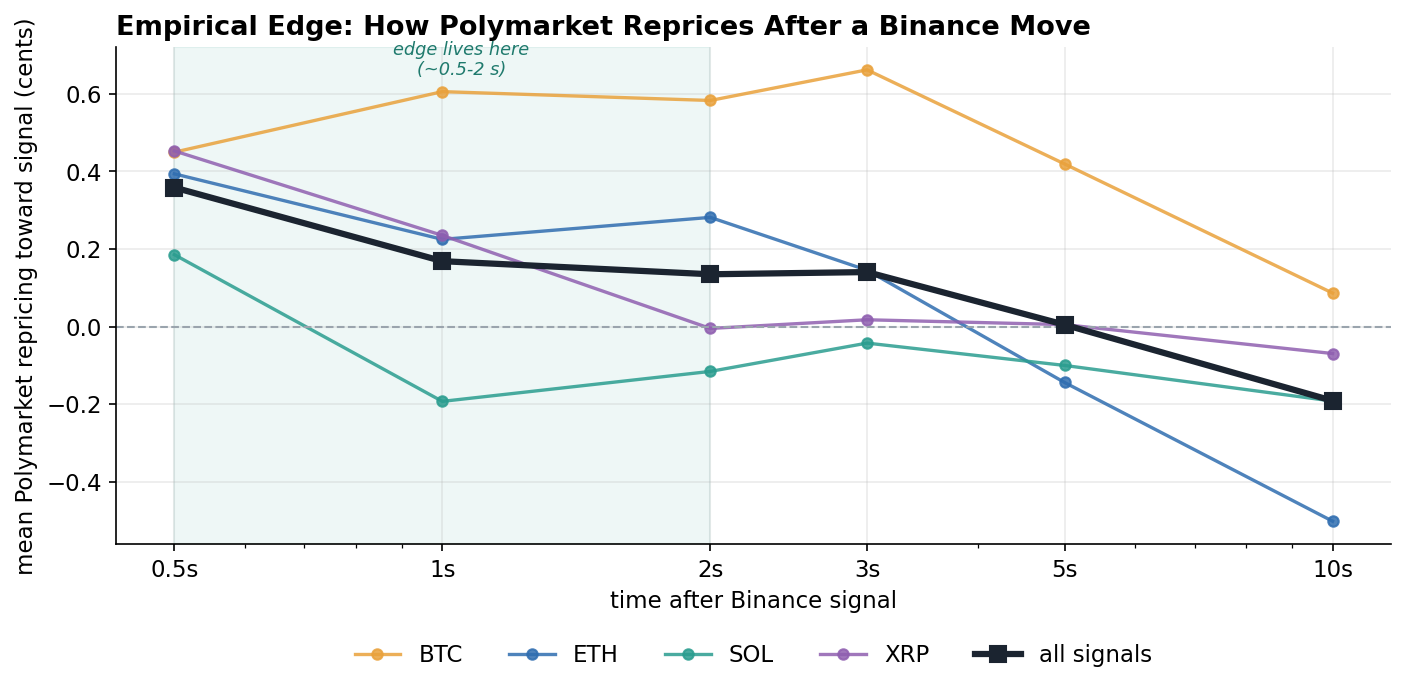
\includegraphics[width=0.86\linewidth]{fig_repricing_curve.png}
  \caption{Empirical Polymarket repricing (in cents, in the signalled direction) at
           fixed horizons after a Binance move, per asset and pooled. The edge is
           concentrated in the first $\sim$2 seconds and reverts by $10$\,s, which
           motivates both the low-latency design and the short holding periods.}
  \label{fig:repricing}
\end{figure}

\subsection{Why the Edge Is Structurally Thin}

The edge is bounded on both sides. On one side, the repricing lag sets the maximum
time the opportunity exists, and Figure~\ref{fig:repricing} shows the useful part is
barely two seconds. On the other, the physical distance between the price source
(Binance, in Asia) and the execution venue (Polymarket, reachable from Europe or the
US) imposes a one-way transit of $\sim$120\,ms on every signal. The system
therefore operates with little margin: it must detect, decide, transmit, re-decide,
sign, and submit inside a window that the transit alone nearly consumes. This
tension, a real but geographically expensive edge, motivated the two-node,
minimal-protocol architecture of Section~\ref{sec:infra}. Whether the remaining
margin is enough is what a live deployment exists to answer.


% =========================================================
\section{Signal Detection (Tokyo)}
\label{sec:detection}

\subsection{The Three-Gate Detector}

Detection runs in Tokyo, as physically close to Binance as AWS placement allows, so
that a move is observed as early as possible. The detector consumes Binance
\texttt{depth10@100ms} book snapshots and the \texttt{@trade} stream for all four
assets, maintains 60 seconds of rolling per-asset metrics (mid, order-flow
imbalance, VWAP, separated buy/sell volume, book imbalance, and a
millisecond-resolution price ring), and evaluates a conjunction of three gates on
every book update. A signal fires only when \emph{all three} pass simultaneously:

\begin{itemize}
  \item \textbf{Gate A (price move).} The Binance mid has moved at least a threshold
        number of basis points over a short lookback (25--150\,ms). This is the
        cheapest test and is evaluated first, so that the $\sim$99\% of ticks with no
        meaningful move exit in a few hundred nanoseconds.
  \item \textbf{Gate B (tick density).} At least a threshold number of book events
        per 100\,ms occurred in the recent window. Real moves arrive as bursts of
        activity; a slow drift on a thin book does not.
  \item \textbf{Gate C (dollar flow).} The signed traded dollar flow over a short
        window confirms the move's direction and exceeds a threshold. Spoofed orders
        can push the mid and generate book events without anyone actually trading;
        requiring confirming \emph{executed} flow filters book-manipulation moves.
\end{itemize}

\noindent A per-asset cooldown (roughly one Polymarket repricing cycle) debounces
the detector so that a single sustained move produces one signal rather than a burst
of them. On a no-signal tick the detector returns in $\sim$400\,ns; the full
signal-to-wire path, including packing and transmission, was budgeted at
50--200\,\textmu s.

\subsection{Confidence Scoring}

When all gates pass, the detector emits a confidence score in $[0,1]$ used
downstream for position sizing and as an entry gate on the Dublin side. The score is
a weighted blend of how far each gate cleared its threshold, normalised so that
$1.0$ corresponds to roughly three times threshold on each axis:
\[
  c \;=\; 0.5\,\underbrace{\min\!\Big(1,\tfrac{|\Delta_{\text{bps}}|}{3\theta_{\text{move}}}\Big)}_{\text{move}}
    \;+\; 0.3\,\underbrace{\min\!\Big(1,\tfrac{\text{flow}}{3\theta_{\text{flow}}}\Big)}_{\text{flow}}
    \;+\; 0.2\,\underbrace{\min\!\Big(1,\tfrac{\text{density}}{3\theta_{\text{td}}}\Big)}_{\text{density}}.
\]
The move term carries the most weight because the magnitude of the Binance move is
the most direct predictor of how far the Polymarket fair value has decoupled from
its displayed price.

\subsection{Per-Asset Calibration}

The four assets differ enough in tick size, volatility, and flow that a single
threshold set is inappropriate. Every gate parameter is therefore calibrated
per asset. Calibration is performed offline by replaying recorded Binance tick and
trade data and using Optuna's TPE sampler (150 trials per asset) to search the joint
detector-and-exit parameter space. To keep each trial cheap, all rolling metrics are
precomputed once at every candidate lookback window (25--250\,ms) so that a trial
reduces to vectorised NumPy indexing plus a short cooldown pass. The objective
rewards signals whose subsequent move persists in the signalled direction and
penalises reversals (``fakeouts''). Table~\ref{tab:calib} shows representative
calibrated values.

\renewcommand{\arraystretch}{1.2}
\begin{table}[H]
  \centering
  \caption{Representative per-asset calibrated parameters (excerpt).}
  \label{tab:calib}
  \begin{tabular}{lccccc}
    \toprule
    \textbf{Asset} & \textbf{Move thr.} & \textbf{Move win.} & \textbf{Flow min.}
      & \textbf{Cooldown} & \textbf{Exit timeout} \\
     & (bps) & (ms) & (USD) & (s) & (s) \\
    \midrule
    BTC & 4.75 & 25 & 15{,}000 & 5.0  & 14 \\
    ETH & 3.75 & 25 & 800      & 4.5  & 27 \\
    SOL & 4.75 & 25 & 11{,}800 & 10.0 & 3  \\
    XRP & 5.00 & 50 & 13{,}800 & 1.0  & 27 \\
    \bottomrule
  \end{tabular}
\end{table}

\subsection{A Meta-Labeling Layer}

Beyond the hand-tuned gates, a second research layer was built: per-asset,
per-timeframe gradient-boosted (LightGBM) and random-forest meta-models trained to
predict whether a raw detector signal would convert into a profitable trade, using
the full microstructure feature vector at signal time (volatility ratios, order-flow
imbalance, book depth, tick and trade rates, and the Polymarket spread and distance
from $0.50$). Filtering a fast, permissive detector with a slower, more selective
model raises precision without slowing the hot path, since the model runs only on the
ticks that already cleared the gates. Its findings are consistent with the
conditional structure documented in Section~\ref{sec:backtest-drivers}.


% =========================================================
\section{Execution Logic (Dublin)}
\label{sec:execution}

The Dublin node turns a directional signal into a filled position. Its design
priority is the inverse of Tokyo's: where Tokyo optimises for the earliest possible
detection, Dublin optimises for \emph{not trading} unless conditions are favourable,
because on a thin edge a bad fill erases many good ones.

\subsection{Entry Gates}

Every incoming signal passes through ten entry gates, checked in order and
short-circuiting on the first failure:

\begin{enumerate}
  \item \textbf{Signal age.} Reject signals older than 500\,ms (the edge is already
        gone).
  \item \textbf{Clock skew.} Reject signals timestamped more than 50\,ms in the
        future (clock desync or corruption).
  \item \textbf{Confidence.} Reject signals below a minimum confidence (0.10).
  \item \textbf{No-trade zone.} Refuse to open within 30\,s of window expiry, where
        resolution risk dominates the repricing edge.
  \item \textbf{Book present.} There must be a live Polymarket book for the target
        token.
  \item \textbf{Spread.} Reject if the Polymarket bid/ask spread exceeds a cap
        ($\sim$4--5\textcent), where crossing costs consume the edge.
  \item \textbf{Book staleness.} Reject if the newest book snapshot is older than
        5\,s.
  \item \textbf{Price bounds.} Only trade when the outcome token's ask is in
        $[0.25, 0.80]$. As Section~\ref{sec:backtest-drivers} shows empirically,
        prices near $0.50$ are close to a coin flip.
  \item \textbf{Dynamic threshold.} A signal-strength-scaled price check.
  \item \textbf{Position and fill.} The slot must be flat, within risk limits, and
        the fill attempt itself must succeed.
\end{enumerate}

\subsection{Order Execution}

Orders are executed as fill-and-kill (FAK) marketable orders, Polymarket's
immediate-or-cancel, which fill at the quoted price or better and cancel any unfilled
remainder. A single FAK priced at the second book level automatically sweeps the top
level first (it is a better price) and then fills into the second, capturing both
levels with one order and no stepping logic. Buys are priced to take displayed
liquidity; sells (closes), where exiting matters more than price, are priced more
aggressively and post a resting good-till-cancelled remainder if the FAK sweep leaves
size unfilled. Polymarket's taker fee for these markets is modelled per contract as
\[
  f(p) \;=\; p \cdot 0.25 \cdot \big(p\,(1-p)\big)^{2},
\]
which peaks near the middle of the price range and vanishes at the tails; the
price-bounds gate is designed partly around it. As Section~\ref{sec:backtest} shows,
fees are the largest cost in this strategy.

\subsection{Exit Paths}

A position is closed by whichever of five conditions fires first:

\begin{enumerate}
  \item \textbf{Stop-loss.} The outcome token's bid has collapsed past a threshold
        (20--30\% of entry).
  \item \textbf{Reversal.} The Binance underlying itself has reversed through a
        per-asset threshold, invalidating the thesis at the source.
  \item \textbf{Convergence.} After a minimum hold ($\sim$3.5\,s), the Polymarket mid
        has moved through entry in our favour and Binance velocity has exhausted.
        This is the intended, profitable exit and accounts for $78\%$ of closes.
  \item \textbf{Timeout.} A per-asset maximum hold (3--27\,s) has elapsed.
  \item \textbf{Emergency.} A 15\,s dead-man timer that force-closes regardless of
        state. As Section~\ref{sec:backtest-drivers} shows, trades that reach this
        timer are the strategy's worst cohort.
\end{enumerate}

\subsection{Sizing and Risk Limits}

Sizing is intentionally small and bounded, appropriate for a strategy whose capacity
is unknown and whose fills are uncertain. Orders default to \$100 notional (also the
per-order cap), with a hard ceiling of 200 contracts per trade. Exposure is capped
at \$500 per asset and \$2{,}000 in aggregate, with no more than 10 open orders at
once. A dual-window rate limiter (a 10-second burst bucket and a 10-minute sustained
bucket, mirroring Polymarket's published limits) gates every API call and always
reserves tokens for closes, so the system can never rate-limit itself out of exiting
a position.


% =========================================================
\section{Infrastructure}
\label{sec:infra}

The infrastructure exists to serve one requirement: move a decision from beside
Binance to beside Polymarket, and act on it, faster than the Polymarket book
reprices. Every design choice below follows from that.

\subsection{Two-Node Topology}

Because Binance and Polymarket are reached from different continents, detection and
execution are split across two nodes (Figure~\ref{fig:arch}). The \textbf{Tokyo}
node does all Binance-facing work and no execution; the \textbf{Dublin} node does
all Polymarket-facing work and no detection. They communicate over a single,
minimal, connectionless link, so that each node is physically close to the venue it
talks to and the expensive intercontinental hop is crossed exactly once, by the
smallest message and as early as possible.

\begin{figure}[H]
  \centering
  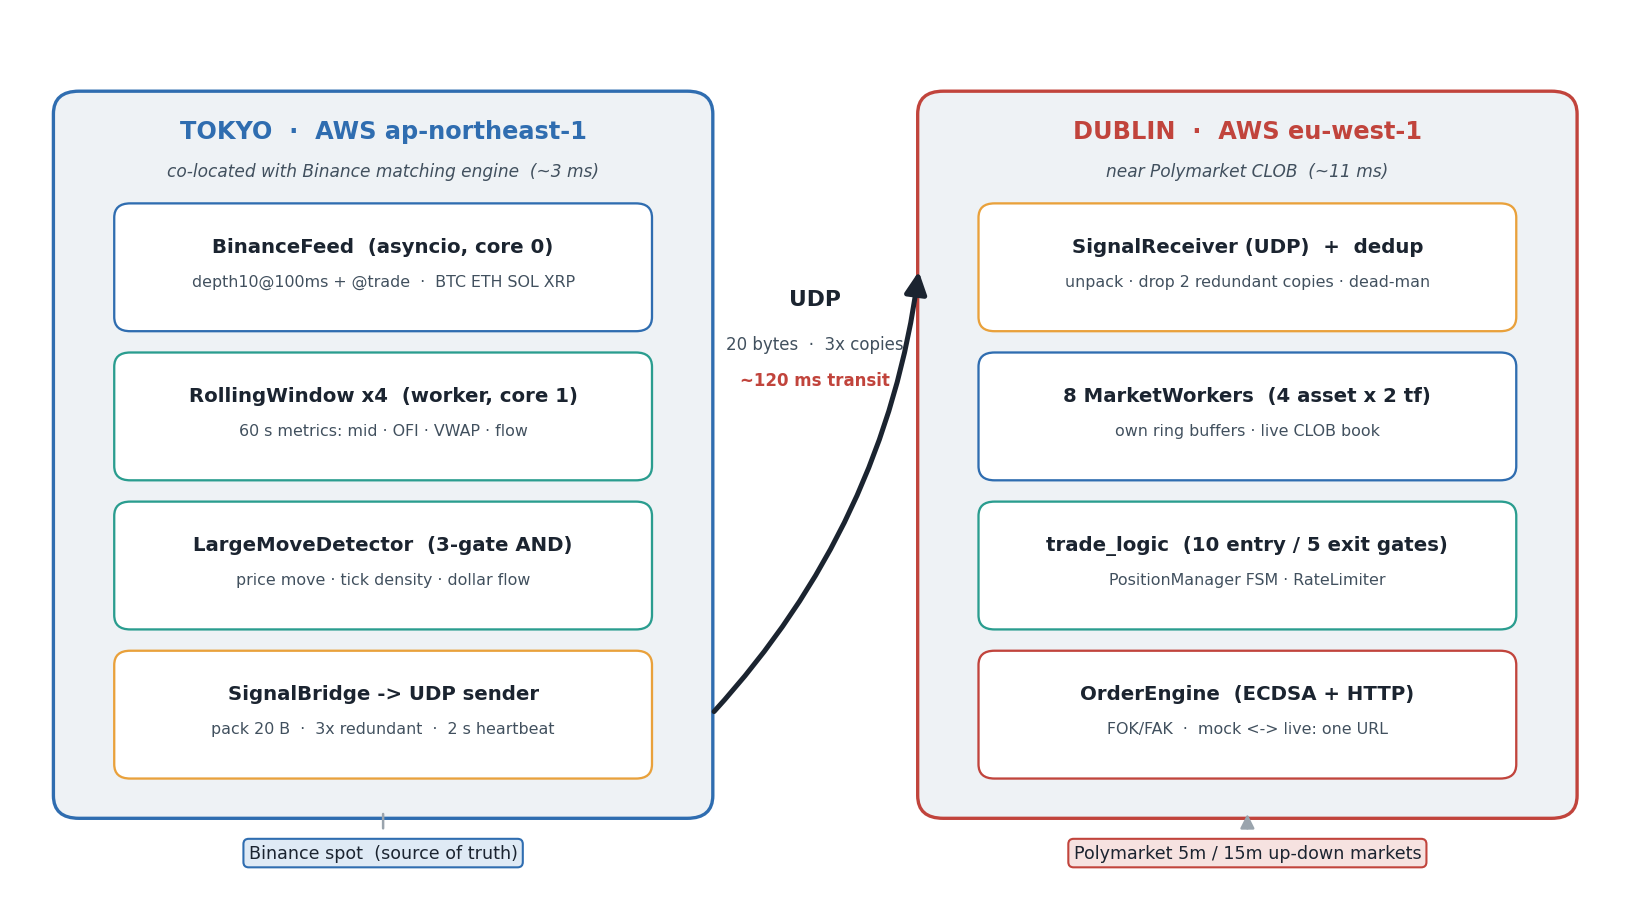
\includegraphics[width=\linewidth]{fig_architecture.png}
  \caption{Two-node architecture. Tokyo detects Binance moves and transmits a
           20-byte UDP signal; Dublin receives, validates against the live
           Polymarket book, and executes. Each node is co-located with the venue it
           serves.}
  \label{fig:arch}
\end{figure}

\subsection{The Wire Protocol}

The link between the nodes is a hand-rolled binary protocol carried over UDP. TCP
was rejected deliberately: a lost packet on a 120\,ms link would trigger a
retransmit that arrives long after the edge is gone, so reliability through
retransmission is worthless here. Instead, each signal is packed into 20 bytes and
sent as \textbf{three redundant copies}; the receiver processes the first to arrive
and discards duplicates by sequence number. This trades a few extra bytes for
resilience to single-packet loss without ever waiting for a round trip. The full
frame is given in Table~\ref{tab:protocol}.

\renewcommand{\arraystretch}{1.2}
\begin{table}[H]
  \centering
  \caption{Signal wire format (20-byte payload, big-endian). One frame carries
           either an OPEN or a CLOSE; bytes 13--14 are repurposed as a reference id
           on CLOSE.}
  \label{tab:protocol}
  \begin{tabular}{clcl}
    \toprule
    \textbf{Offset} & \textbf{Field} & \textbf{Bytes} & \textbf{Description} \\
    \midrule
    0  & magic        & 1 & \texttt{0xA7} marks a valid packet \\
    1  & seq          & 2 & sequence number (wraps at 65535) \\
    3  & copy\_id     & 1 & redundant copy index (0, 1, 2) \\
    4  & timestamp    & 8 & epoch microseconds \\
    12 & flags        & 1 & bit-packed (below) \\
    13 & magnitude    & 1 & OPEN: move in bps / CLOSE: ref id high \\
    14 & confidence   & 1 & OPEN: score 0--255 / CLOSE: ref id low \\
    15 & price        & 4 & Binance price $\times\,10{,}000$ \\
    19 & checksum     & 1 & XOR of bytes 0--18 \\
    \bottomrule
  \end{tabular}
\end{table}

\noindent The single \texttt{flags} byte packs everything needed to route and
interpret the signal: a debug bit, a two-bit close reason, a two-bit asset selector,
a direction bit, and an action bit. A separate heartbeat frame (magic \texttt{0xA8},
sent every 2\,s) lets Dublin detect if Tokyo goes dark: if heartbeats stop, Dublin
knows no signals are coming and existing positions ride out their timeouts safely.
When Tokyo sets the debug bit, Dublin forces paper mode and captures extended
diagnostics, so a single flag on the sending side switches the whole system between
live and instrumented dry-run.

\subsection{Node-Internal Design}

Both nodes follow the same discipline: the thread doing network I/O never does heavy
computation, and the thread doing computation never does I/O, with a single
non-blocking queue between them. \textbf{Tokyo} runs an asyncio event loop on one
core (Binance WebSockets in, status logging) and a worker thread on another (four
rolling-window detectors, exit monitoring, signal packing, UDP send); handoff is an
$O(1)$ \texttt{put\_nowait} that can never block the feed. \textbf{Dublin} runs all
WebSocket feeds (the Polymarket CLOB, the relayed Binance/Chainlink price stream,
and the user fill channel) on its asyncio core, and eight worker threads (one per
(asset, timeframe) slot) on the other, each owning its own pre-allocated numpy ring
buffers so that no worker ever contends with another for its market's data. Per-slot
position state is a small explicit finite state machine
(\texttt{FLAT} $\rightarrow$ \texttt{OPENING} $\rightarrow$ \texttt{LONG/SHORT}
$\rightarrow$ \texttt{CLOSING} $\rightarrow$ \texttt{FLAT}) locked across the
two-phase submit/resolve of every order, which makes concurrent duplicate opens
structurally impossible.

\subsection{Mock-to-Live Parity}

A standalone mock CLOB server replicates Polymarket's HTTP and WebSocket API: the
same order endpoints, the same 200-status-with-error-body convention, the same
published rate limits, and, most importantly, order books populated from
\emph{Polymarket's real market data feed}. The mock subscribes to the live
Polymarket book over WebSocket and simulates fills by walking the displayed levels.
The entire Dublin system talks to the mock or to production through the same code
path; going live is a single change of host URL, with no code change. This parity
was a deliberate engineering goal, and it succeeded technically. It also,
unavoidably, reproduced the market's blind spot, the subject of
Section~\ref{sec:postmortem}.

\subsection{Latency Budget}

Figure~\ref{fig:latency} decomposes the measured end-to-end path. Detection near
Binance costs $\sim$3\,ms; in-node compute in Tokyo is sub-millisecond; the UDP hop
to Dublin is $\sim$120\,ms; Dublin's gate evaluation and ECDSA order signing add a
few milliseconds; and the order reaches Polymarket in $\sim$11\,ms. The total,
$\sim$140--150\,ms, sits at the fast end of the repricing window. The system was
fast enough, but the transatlantic segment consumes most of the budget, and no local
optimisation can shrink it.

\begin{figure}[H]
  \centering
  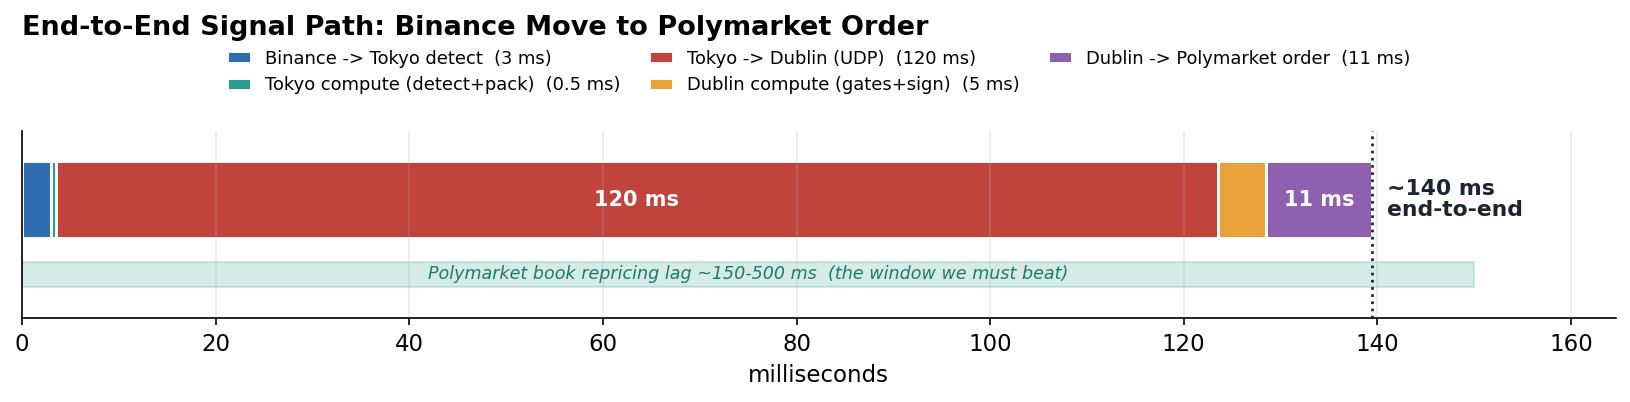
\includegraphics[width=\linewidth]{fig_latency_budget.png}
  \caption{Measured end-to-end latency from a Binance move to a Polymarket order.
           The $\sim$120\,ms Tokyo$\rightarrow$Dublin transit dominates; all
           node-internal compute together is a few milliseconds.}
  \label{fig:latency}
\end{figure}


% =========================================================
\section{Deployment}
\label{sec:deployment}

\subsection{Instances and Placement}

The system ran on two AWS \texttt{c6a.large} instances (2 vCPU each, roughly \$52 per
month on-demand), one in \texttt{ap-northeast-1} (Tokyo) and one in
\texttt{eu-west-1} (Dublin). ``Co-location'' here means region and
availability-zone placement in the same metro as each venue, with connectivity over
AWS's internal backbone rather than the public internet. That backbone gives lower
and, more importantly, lower-jitter latency than a commodity path, without the cost
or lead time of true datacenter cross-connects. Two vCPUs matches each node's
two-core design: one core for I/O, one for compute, pinned explicitly. The whole
system cost roughly \$100/month to run.

\subsection{Measured Latencies}

From the deployed nodes, the measured characteristics were approximately 3\,ms from
Tokyo to Binance, 120\,ms from Tokyo to Dublin, and 11\,ms from Dublin to
Polymarket. These are the numbers behind the budget in Figure~\ref{fig:latency}, and
they held stably enough that transit variance was never the binding constraint.

\subsection{Operations}

Each node logs a compact status line at a fixed interval: Tokyo every 5\,s (queue
depth, signals sent/dropped, per-asset mid, order-flow imbalance, recent move, book
imbalance), Dublin every 15\,s (fills, cancels, timeouts, exposure, realised P\&L,
open orders, rate-limit headroom, heartbeat age). Every state change is written to a
dual JSONL-and-parquet trade log, and a post-session analyser computes P\&L,
win-rate, per-asset breakdown, and exit-reason distribution from the log at
shutdown. The debug flag adds per-event timing histograms and full book-state
captures at signal time, at zero overhead when disabled.


% =========================================================
\section{Backtest Performance}
\label{sec:backtest}

The results in this section come from replaying the full strategy (detection, gates,
execution logic, fees, and exits) over $13$ recorded feed sessions
($8{,}576$ trades across roughly $52$ hours of order flow). The analysis is confined
to the 5-minute markets, which is deliberate rather than a limitation: the large
majority of the backtested P\&L came from the 5-minute windows, where the higher
window-rotation frequency produces more repricing events per hour than the 15-minute
markets. Fills are simulated against the recorded Polymarket book. As
Section~\ref{sec:postmortem} explains, that fill assumption is what did not hold
live; these numbers therefore describe the strategy's behaviour \emph{given} that
displayed liquidity is real, which is the right way to read every figure below.

\subsection{Headline Results}

The strategy won $61.4\%$ of its $8{,}576$ trades, with a median holding period of
$7.6$\,s. The per-trade net P\&L distribution (Figure~\ref{fig:pnldist}) is centred
just above zero and positively skewed, consistent with a small, repeatable edge
rather than occasional large wins. Exits were dominated by the intended convergence
path ($78\%$), with the remainder split across emergency timeouts ($16\%$),
opposite-signal closes ($4\%$), and stop-losses ($2\%$).

\begin{figure}[H]
  \centering
  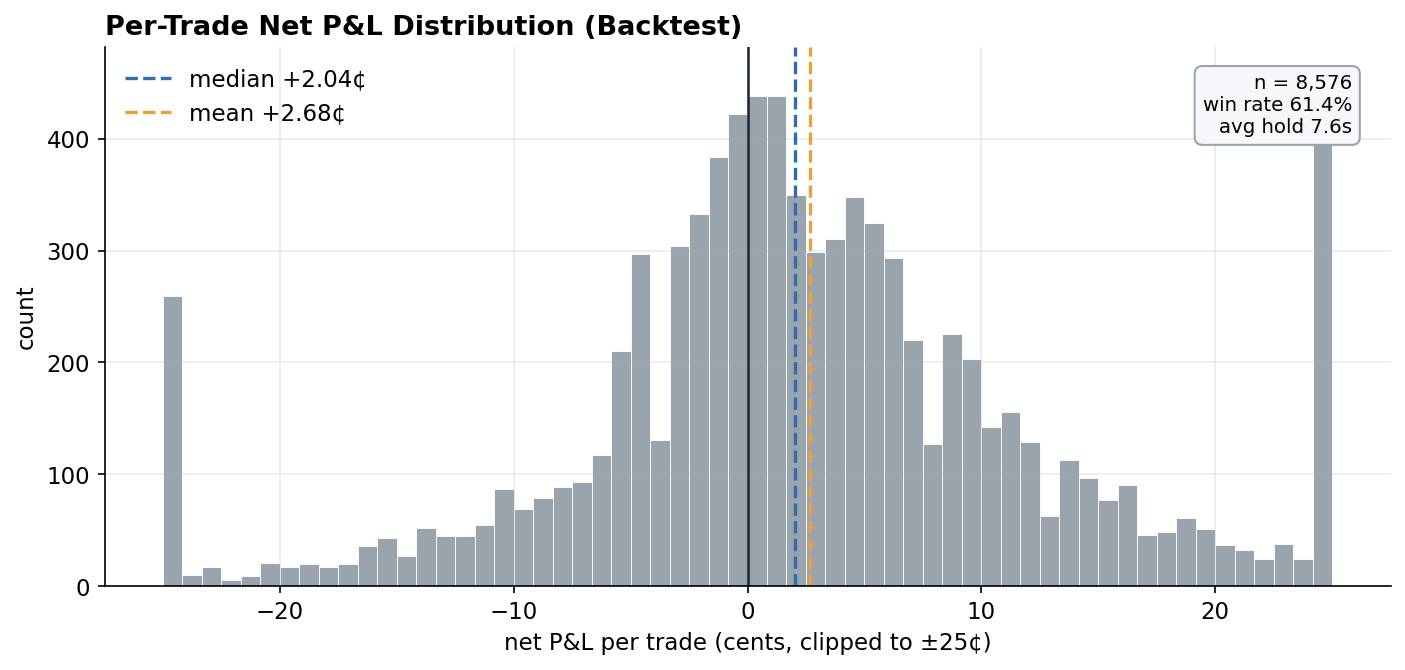
\includegraphics[width=0.82\linewidth]{fig_pnl_distribution.png}
  \caption{Per-trade net P\&L (cents, clipped to $\pm25$\textcent\ for display).
           Positive mean and median, $61.4\%$ win rate, across $8{,}576$ trades.}
  \label{fig:pnldist}
\end{figure}

\subsection{Fees Dominate}

The most notable feature of the equity curve (Figure~\ref{fig:equity}) is the gap
between gross and net. The strategy earned $+51{,}350$\textcent\ gross but paid
$28{,}403$\textcent\ in fees ($55\%$ of gross), leaving $+22{,}948$\textcent\ net.
This is the basic arithmetic of a high-turnover strategy on a sub-cent edge: even at
Polymarket's fee schedule, more than half of every unit of gross edge is consumed at
the point of execution. It also sets a demanding bar for live execution, since any
degradation in fill quality comes directly out of the thin margin that survives fees.

\begin{figure}[H]
  \centering
  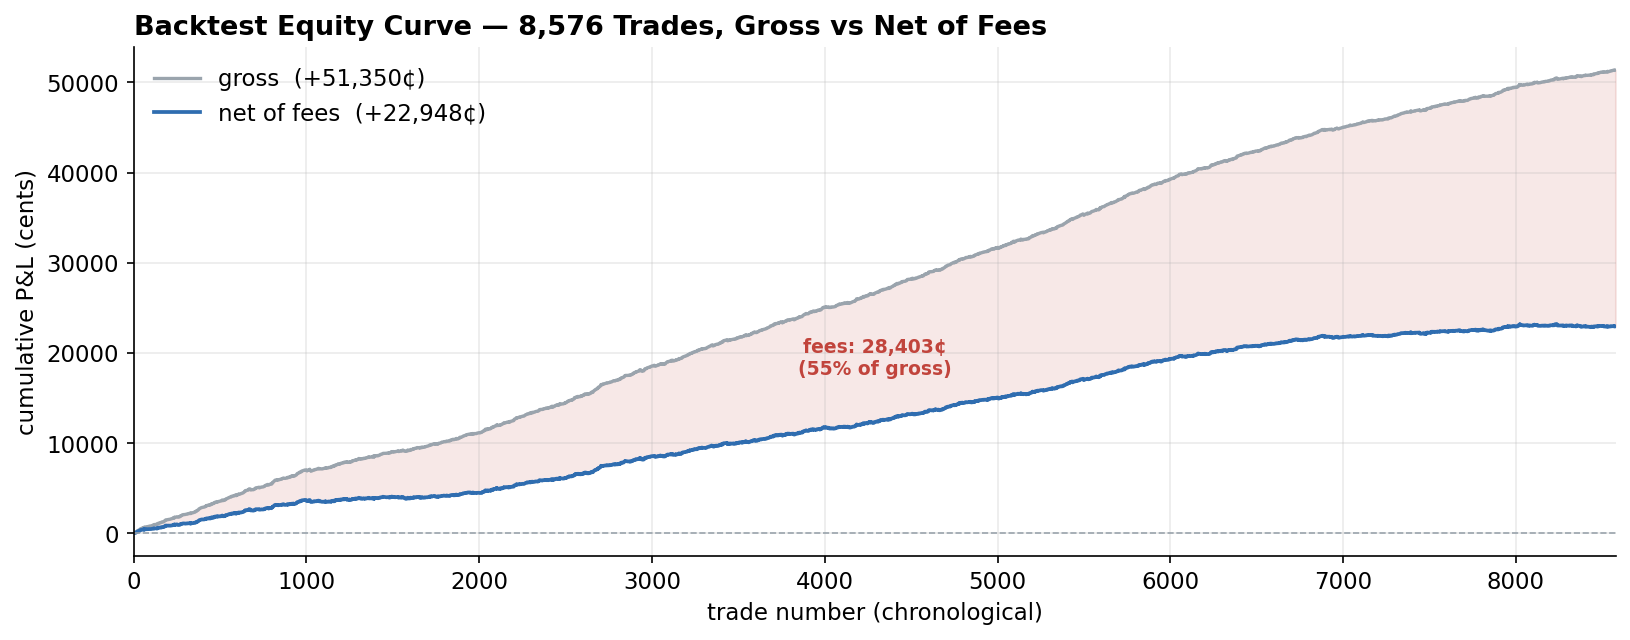
\includegraphics[width=\linewidth]{fig_equity_curve.png}
  \caption{Backtest equity curve over $8{,}576$ chronological trades. Gross P\&L
           (grey) rises steadily; fees (shaded) consume $55\%$ of it, leaving the net
           curve (blue). The edge is real; the fee drag is large.}
  \label{fig:equity}
\end{figure}

\subsection{The Edge Has Structure}
\label{sec:backtest-drivers}

The edge varies systematically with conditions the strategy can observe at entry
(Figure~\ref{fig:drivers}), and each relationship has a microstructural reading.

\begin{itemize}
  \item \textbf{Tick rate (panel a).} Win rate falls monotonically from $68\%$ in
        quiet books ($<30$ ticks/s) to a losing $49\%$ in the fastest ($>300$
        ticks/s). Section~\ref{sec:tickrate} decomposes the cause.
  \item \textbf{Distance from $0.50$ (panel b).} Near $0.50$ the outcome is close to
        a coin flip ($51\%$); the edge strengthens toward the wings ($65$--$68\%$),
        where the token price is more sensitive to the underlying and the fair-value
        decoupling from a Binance move is larger.
  \item \textbf{Hold time (panel c).} P\&L is sharply bimodal. The profitable cohorts
        exit at $2$--$5$\,s ($+19{,}774$\textcent) and $8$--$12$\,s
        ($+14{,}243$\textcent); the trades that run to the $12$--$20$\,s
        emergency-timeout band are heavily negative ($-10{,}531$\textcent). This is
        the same $\sim$2\,s edge horizon seen in Figure~\ref{fig:repricing}: hold
        past it and the position is systematically underwater.
  \item \textbf{Asset (panel d).} All four assets were net profitable in replay, with
        SOL and XRP posting the highest win rates ($\sim$65\%) and BTC/ETH the
        largest absolute P\&L.
\end{itemize}

\begin{figure}[H]
  \centering
  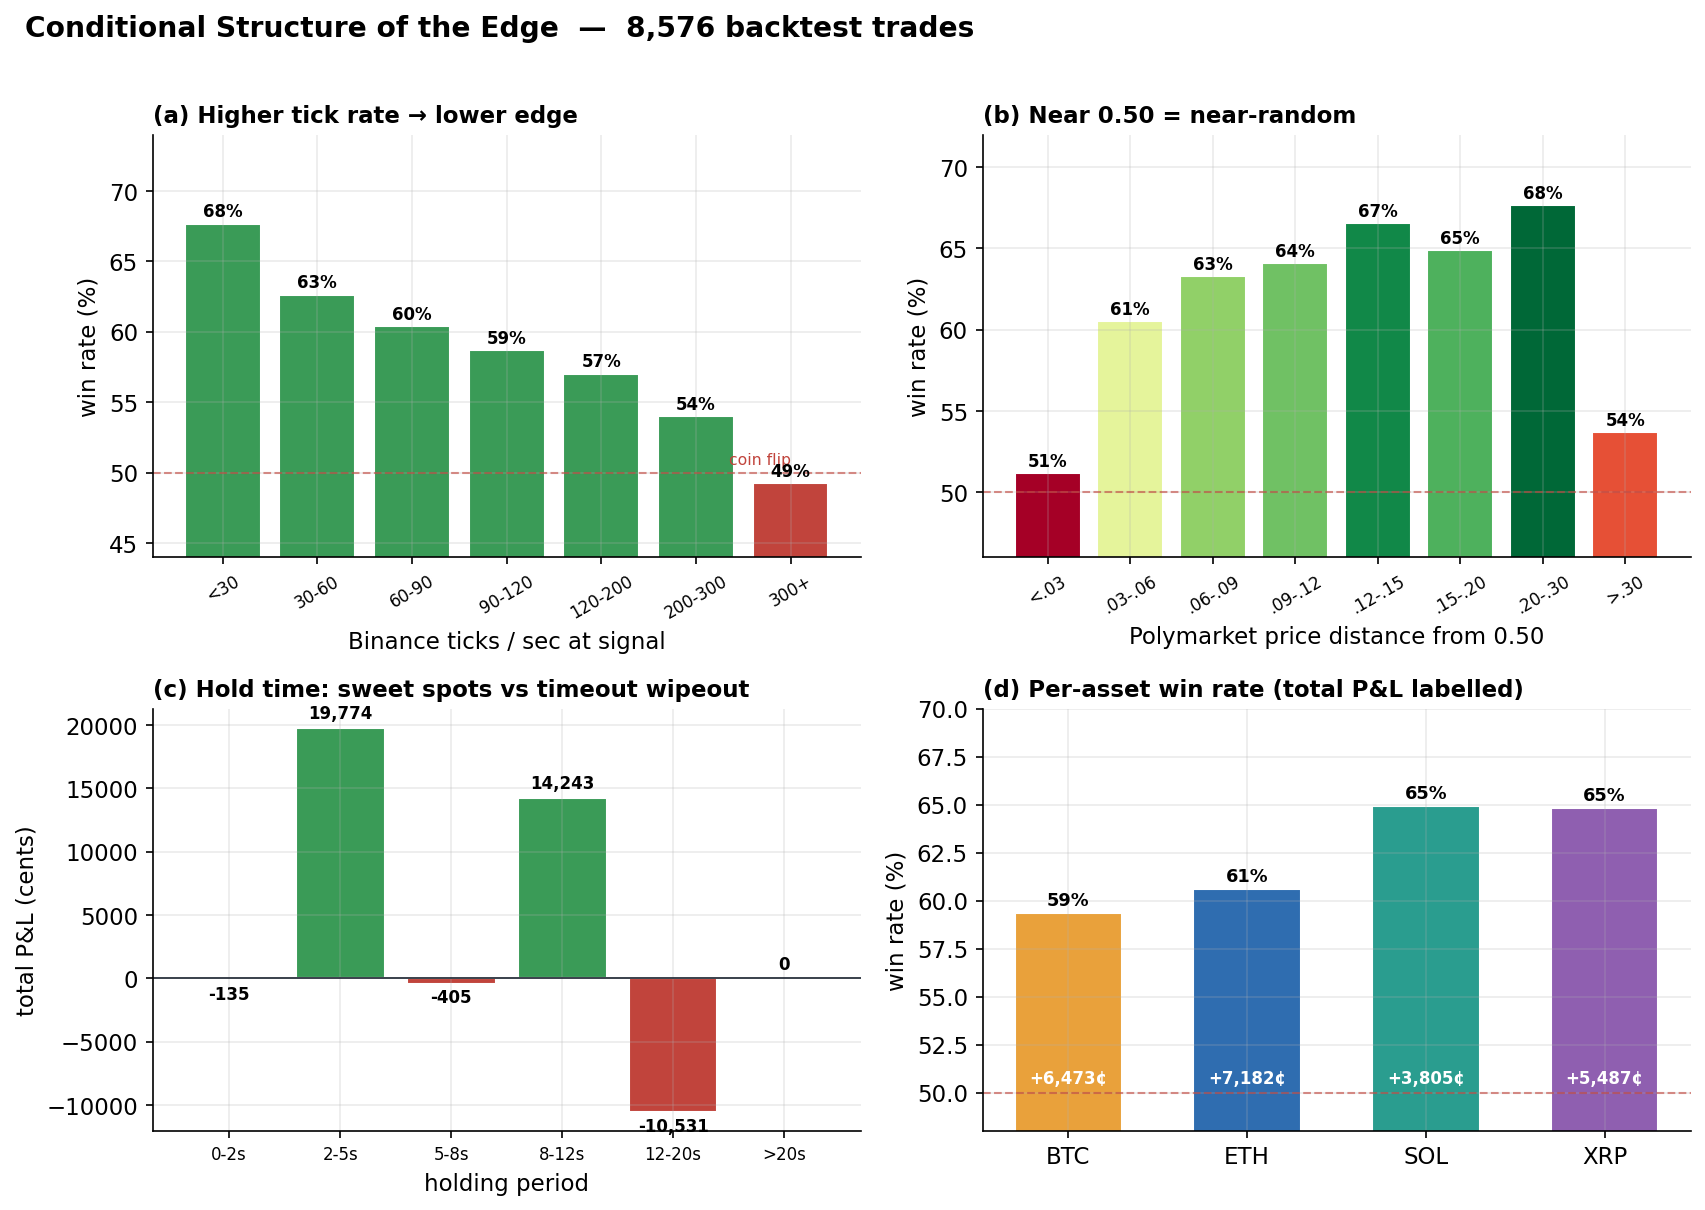
\includegraphics[width=\linewidth]{fig_edge_drivers.png}
  \caption{Conditional structure of the edge across $8{,}576$ backtest trades. The
           edge concentrates in quiet books, away from $0.50$, at short holding
           periods, and inverts in each opposite condition.}
  \label{fig:drivers}
\end{figure}

\noindent These are the properties of a healthy microstructure edge: profitable on
average, coherent in its drivers, and consistent with the measured repricing
dynamics. That is what made the live outcome informative.

\subsection{Why the Tick-Rate Effect: Reversal, Not Throughput}
\label{sec:tickrate}

The tick-rate relationship (panel a above) is the strongest and most actionable of
the four, so its cause is worth isolating. One candidate explanation is throughput:
that the system cannot keep up when the Binance feed is fast. The data rules this
out. The relationship appears in the \emph{replay} backtest, which processes every
recorded tick and does not model the live event queue at all; if it were a throughput
artefact, it could not appear here. The cause is therefore in the market, and
Figure~\ref{fig:tickrate} shows it has two parts.

\begin{figure}[H]
  \centering
  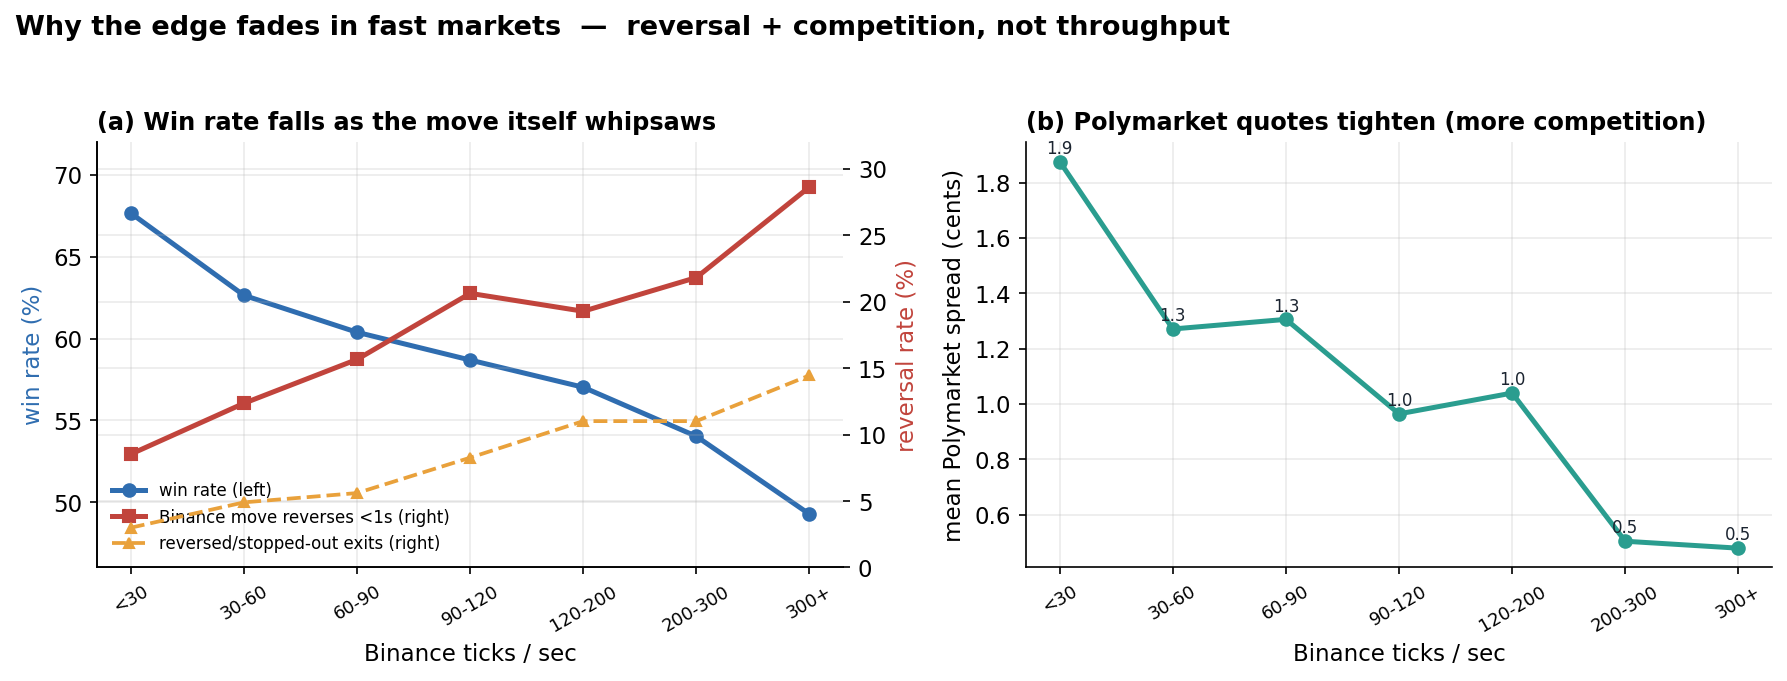
\includegraphics[width=\linewidth]{fig_tickrate_mechanism.png}
  \caption{Decomposing the tick-rate effect. (a) Win rate (blue) is almost a mirror
           image of how often the triggering Binance move reverses within one second
           (red). The moves are not larger at high tick rate ($\sim$2.2\,bps
           throughout), only more likely to reverse, so reversed and stopped-out
           exits (amber) climb with it. (b) The Polymarket spread tightens from
           $\sim$1.9\textcent\ to $\sim$0.5\textcent\ as activity rises, evidence of
           more competitive quoting.}
  \label{fig:tickrate}
\end{figure}

\noindent \textbf{Adverse selection at the source} is the dominant part. In quiet
books ($<30$ ticks/s) the triggering move reverses within a second only $8.5\%$ of
the time; in the fastest ($>300$ ticks/s) it reverses $28.6\%$ of the time, a
$3.4\times$ increase. Since the move magnitude is essentially flat across the range,
fast-market signals are more likely to be transient liquidity spikes that snap back,
and following momentum into them is adversely selected. That is why reversed and
stopped-out exits rise from $\sim$3\% to $\sim$14\% over the same range.

\medskip
\noindent \textbf{Competition} is the secondary part. As Binance activity rises, the
Polymarket book is quoted more tightly (the mean spread falls from $\sim$1.9\textcent\
to $\sim$0.5\textcent) because more market-makers and competing latency arbitrageurs
are active, leaving a smaller and shorter-lived mispricing to capture. The practical
consequence is that the $<100$ ticks/s gate the strategy already applies is
well-founded; the data would further support scaling size down, rather than trading
flat, above $\sim$120 ticks/s.


% =========================================================
\section{Production Results and Post-Mortem}
\label{sec:postmortem}

\subsection{What Happened}

In paper trading against the mock CLOB, the system performed as
Section~\ref{sec:backtest} describes. Signals fired at sensible rates, gates rejected
stale and thin conditions, and marketable orders filled at essentially $100\%$. The
mock filled any order the displayed book could satisfy, and the displayed book always
appeared deep enough. Live, with real capital, roughly \textbf{one order in ten
filled}. Same signals, same gates, same latency. Nine times out of ten, the liquidity
shown on the book was gone by the time the order arrived. The orders that did fill
were close to coin flips, so the live deployment came out effectively flat: it did not
lose money, but it did not capture the backtested edge either.

\subsection{Root Cause: Spoofed Liquidity}

The displayed depth on the Polymarket book was, to a large extent, not real. Resting
orders that made the book look deep were cancelled the instant a real order tried to
cross them: classic spoofing, and especially effective in a low-participation venue
where a few actors can shape the whole visible book. The strategy's premise was to
\emph{take} that displayed liquidity during the repricing window. When the liquidity
was a bluff, there was nothing to take: the FAK order arrived, found the quoted size
withdrawn, filled a token amount or nothing, and cancelled the rest.

\medskip
\noindent This failure mode was invisible in paper by construction. The mock CLOB
simulated fills by walking the \emph{displayed} book levels, the same book the
spoofers controlled. It had no model of cancellation-on-arrival because the real book
gives no advance signal of it; the cancellation is a \emph{reaction} to the arriving
order, and no amount of pre-trade book data contains it. The paper harness was
faithful to the displayed market and therefore inherited the same deception. The more
realistic the mock was made (consuming displayed liquidity, enforcing real rate
limits, using the real feed), the more convincingly it reproduced the illusion. Every
favourable number in Section~\ref{sec:backtest} rests on this one false assumption.

\subsection{Why Latency Was Not the Problem}

It is useful to separate what failed from what did not. The signal was predictive
(Figure~\ref{fig:repricing}). The backtest was profitable with coherent structure
(Figures~\ref{fig:equity}--\ref{fig:drivers}). The latency budget was met
(Figure~\ref{fig:latency}). The engineering was correct: the system did what it was
built to do, on time. The strategy still could not make money, because a latency
arbitrage implicitly assumes that winning the race entitles you to the liquidity at
the finish line, and in this venue it did not.

\subsection{Adverse Selection, Restated}

Seen through a market-microstructure lens, the fills the system \emph{did} get were
adversely selected. On the occasions liquidity did not vanish, it often did not
vanish because the resting side was willing to trade, which is disproportionately the
case when that side is better informed or the move is about to reverse. The strategy
was thus filled mainly when being filled was worst, and starved when being filled
would have been best. The fills that did occur were therefore close to a coin flip,
which is why the live deployment came out flat rather than either profitable or
loss-making. A displayed-book backtest cannot represent this, because it
fills every order symmetrically regardless of why the counterparty is or is not
there.


% =========================================================
\section{Lessons and What I Would Do Differently}

\subsection{Validate Liquidity, Not Just Signal}

The main error was validating the signal thoroughly while assuming the execution
surface. A corrected process would treat \emph{realisable} liquidity as a
first-class unknown to be measured, not inferred from the screen. Concretely: before
committing capital, run a campaign of small live probe orders across the target
markets and measure the empirical fill rate as a function of displayed size, order
aggressiveness, and time-of-day; compare displayed depth against depth that actually
transacts in the historical trade prints; and treat any market where realised fills
fall far short of displayed depth as untradeable by a liquidity-taking strategy,
however attractive the signal.

\subsection{Model Cancellation-on-Arrival}

A paper harness for a liquidity-taking strategy must include a fill model that can
decline. Even a crude one (filling a displayed level only with some probability, or
applying a haircut calibrated to observed live fill rates) would have collapsed the
$61\%$-win-rate backtest to break-even or worse and prevented the deployment. The point
generalises: a backtest that fills against displayed depth is only valid for
liquidity-\emph{providing} strategies; for liquidity-takers it is systematically
optimistic and must be corrected with a realistic, ideally empirically-calibrated,
fill model.

\subsection{Respect the Geography}

The $\sim$120\,ms transatlantic hop was the hard floor of this design, and it left
almost no margin against a $\sim$2\,s edge. Where the price source and execution
venue are far apart, that transit cost should be the first number computed, and a
strategy should proceed only if its edge comfortably survives it, not merely fits
inside it.

\subsection{Where This Approach Does Work}

None of this invalidates cross-venue latency arbitrage as a class. It works when the
liquidity being raced toward is firm: deep, professionally market-made venues where
displayed size is largely real and cancellation-on-arrival is the exception. The
infrastructure built here (the two-node split, the minimal UDP protocol, the
shared-nothing per-asset pipelines, the mock-to-live parity, and the calibration and
meta-labeling stack) is sound and reusable. What must change is the target: a venue
whose book can be trusted, or a strategy that provides liquidity rather than taking
it.


% =========================================================
\section{Conclusion}

This was a complete, deployed, real-money low-latency trading system built around a
real and empirically validated inefficiency, and it failed for a reason that none of
the engineering it demonstrates could have fixed. The signal predicted short-horizon
repricing; the backtest was profitable with coherent conditional structure; the
infrastructure delivered orders inside the repricing window; the deployment was
cheap, stable, and correct. The strategy still made no money, because the liquidity it
was designed to capture was largely illusory, and because the paper harness, faithful
to the displayed book, could not detect this until real capital met the real book. It
did not lose money; the backtested edge simply did not survive live execution, and the
deployment was retired flat.

\medskip
\noindent The engineering artefacts retain their value: a template for co-located
two-node systems, a compact loss-tolerant signalling protocol, a disciplined
shared-nothing processing model, and a mock-to-live harness with faithful API parity. The
strategic lesson is more portable than any of them. In a latency arbitrage, speed is
necessary but not sufficient; the binding question is whether the liquidity at the
end of the race is real. On Polymarket's short-dated crypto markets, in this period,
for a liquidity-taker, it was not. Establishing that with a small, well-instrumented,
inexpensive deployment rather than a large one is the useful result here.


\appendix
% =========================================================
\section{System Reference}

\subsection{Component Map}

\renewcommand{\arraystretch}{1.2}
\begin{longtable}{L{3.2cm} L{2.0cm} L{9.0cm}}
  \caption{Principal components by node.} \label{tab:components} \\
  \toprule
  \textbf{Component} & \textbf{Node} & \textbf{Responsibility} \\
  \midrule
  \endfirsthead
  \multicolumn{3}{c}{{\bfseries Table \thetable\ continued}} \\
  \toprule
  \textbf{Component} & \textbf{Node} & \textbf{Responsibility} \\
  \midrule
  \endhead
  \bottomrule
  \endfoot
  \bottomrule
  \endlastfoot
  BinanceFeed        & Tokyo  & Binance depth + trade WebSocket ingest; inter-snapshot book estimation \\
  RollingWindow      & Tokyo  & 60\,s per-asset metrics (mid, OFI, VWAP, flow, imbalance, price ring) \\
  LargeMoveDetector  & Tokyo  & Three-gate signal detection and confidence scoring \\
  ExitMonitor        & Tokyo  & Tracks active signals; emits CLOSE on reversal/timeout \\
  SignalBridge / Sender & Tokyo & Packs 20-byte frames; sends 3 redundant UDP copies; heartbeat \\
  SignalReceiver     & Dublin & UDP ingest; sequence-based dedup; dead-man detection \\
  PolyClobFeed       & Dublin & Polymarket CLOB book/trade WebSocket; window rotation \\
  MarketWorker ($\times$8) & Dublin & Per-(asset, timeframe) event processing over private ring buffers \\
  trade\_logic       & Dublin & Ten entry gates, five exit paths \\
  OrderEngine / Executor & Dublin & ECDSA signing; FAK/FOK execution; fill reconciliation \\
  PositionManager / FSM & Dublin & Per-slot state machine; two-phase open/close; risk gating \\
  RateLimiter        & Dublin & Dual-window API limiter with close reserve \\
\end{longtable}

\subsection{Backtest Summary}

\renewcommand{\arraystretch}{1.2}
\begin{table}[H]
  \centering
  \caption{Replay backtest summary (paper fill assumption).}
  \label{tab:backtest}
  \begin{tabular}{ll}
    \toprule
    \textbf{Metric} & \textbf{Value} \\
    \midrule
    Trades                 & 8{,}576 \\
    Recorded sessions      & 13 ($\sim$52 hours, 5m markets) \\
    Win rate               & 61.4\% \\
    Median hold            & 7.6\,s \\
    Gross P\&L             & $+51{,}350$\textcent \\
    Fees                   & $28{,}403$\textcent\ (55\% of gross) \\
    Net P\&L               & $+22{,}948$\textcent \\
    Convergence exits      & 78\% \\
    Emergency / opp.\ / stop & 16\% / 4\% / 2\% \\
    Repricing half-life    & $\sim$786\,ms (median) \\
    \midrule
    \textbf{Live fill rate} & \textbf{$\sim$10\% (vs $\sim$100\% paper)} \\
    \textbf{Live outcome}   & \textbf{effectively flat} \\
    \bottomrule
  \end{tabular}
\end{table}

\subsection{Key Parameters}

\renewcommand{\arraystretch}{1.2}
\begin{table}[H]
  \centering
  \caption{Selected system parameters.}
  \label{tab:params}
  \begin{tabular}{lll}
    \toprule
    \textbf{Parameter} & \textbf{Value} & \textbf{Where} \\
    \midrule
    Assets                & BTC, ETH, SOL, XRP        & both \\
    Timeframes            & 5\,min, 15\,min           & Dublin \\
    Detector lookback     & 25--150\,ms               & Tokyo \\
    Signal packet size    & 20 bytes ($\times$3 copies) & wire \\
    Heartbeat interval    & 2\,s                      & wire \\
    Signal-to-wire budget & 50--200\,\textmu s        & Tokyo \\
    Max signal age gate   & 500\,ms                   & Dublin \\
    Price-bounds gate     & $[0.25, 0.80]$            & Dublin \\
    Default order size    & \$100 (cap \$100)         & Dublin \\
    Exposure caps         & \$500 / asset, \$2{,}000 total & Dublin \\
    Emergency dead-man    & 15\,s                     & Dublin \\
    Instances             & 2 $\times$ c6a.large (2 vCPU) & AWS \\
    Regions               & ap-northeast-1, eu-west-1 & AWS \\
    End-to-end latency    & $\sim$140--150\,ms        & measured \\
    Monthly cost          & $\sim$\$100               & AWS \\
    \bottomrule
  \end{tabular}
\end{table}

\end{document}
